\documentclass[11pt]{article}
\usepackage[italian]{babel}
\usepackage[utf8]{inputenc}
\usepackage{graphicx}
\usepackage{float}
\usepackage{amsmath}
\usepackage{amsfonts}
\usepackage{hyperref}
\usepackage{glossaries}
%\makeglossaries
%\newglossaryentry{magic}{
%    name={magic number},
%    description={quel numero che metti in una variabile quando è nulla ma non hai il null. Tipo -1}
%}

\usepackage[normalem]{ulem}
\newcommand{\code}[1]{\texttt{#1}}
\newcommand{\numpy}{{\tt numpy}}    % tt font for numpy
\topmargin -.5in
\textheight 9in
\oddsidemargin -.25in
\evensidemargin -.25in
\textwidth 7in
\begin{document}

% ========== Edit your name here
\author{Simone Montali\\monta.li}
\title{Riassunti di Tecnologie Internet}

\maketitle

\medskip
\section{Internet}
\subsection{HTTP}
Il \textbf{World Wide Web} è uno spazio di informazioni basato su internet, dove documenti e risorse sono identificati da indirizzi. Una \textbf{pagina web} è un documento HTML linkato ad altre pagine/risorse.
Gli \textbf{URI} (\textit{Uniform Resource Identifiers}) sono utilizzati in HTTP come mezzo identificativo delle risorse. 
\begin{center}
    \code{$schema:[//[user:password@]host[:port]][/]path[?query][\#fragment]$}
\end{center}
\textbf{HyperTezt Transfer Protocol} è un protocollo a livello applicativo, che adotta un modello client/server: uno \textbf{user agent} che inizia la connessione HTTP ed invia richieste, e un \textbf{origin server} che accetta le richieste e possiede le risorse. È inoltre utile definire altri tre termini:
\begin{itemize}
    \item \textbf{Local cache}: memoria locale (server o client)
    \item \textbf{Proxy}: applicazione intermediaria avente funzionalità server e client 
    \item \textbf{Gateway}: applicazione intermediaria che lavora per conto del server, senza renderlo noto ai client 
\end{itemize}
\subsubsection{Caratteristiche di HTTP}
\begin{itemize}
    \item \textbf{HTTP utilizza TCP}: il client inizia una connessione TCP (crea la socket) sul server, che accetta e comincia a scambiare messaggi, poi viene chiusa.
    \item \textbf{HTTP è stateless}: il server non mantiene informazioni riguardanti richieste passate 
\end{itemize}
Distinguiamo tra HTTP non-persistent, dove abbiamo un invio di risorsa alla volta, e persistent HTTP, dove più risorse vengono inviate attraverso una singola connessione TCP. Consideriamo il cosiddetto \textbf{Round Trip Time} (RTT): nella prima sono richiesti 2 RTT per risorsa (apertura connessione, invio risorsa), mentre la seconda lascia la connessione aperta, e quindi riduce il numero di RTT richieste. Inoltre, la seconda permette il \textbf{pipelining}, ossia l'invio di più richieste alla volta allo scopo di ridurre i tempi, senza attendere le risposte.
\begin{figure}[H]
    \centering
    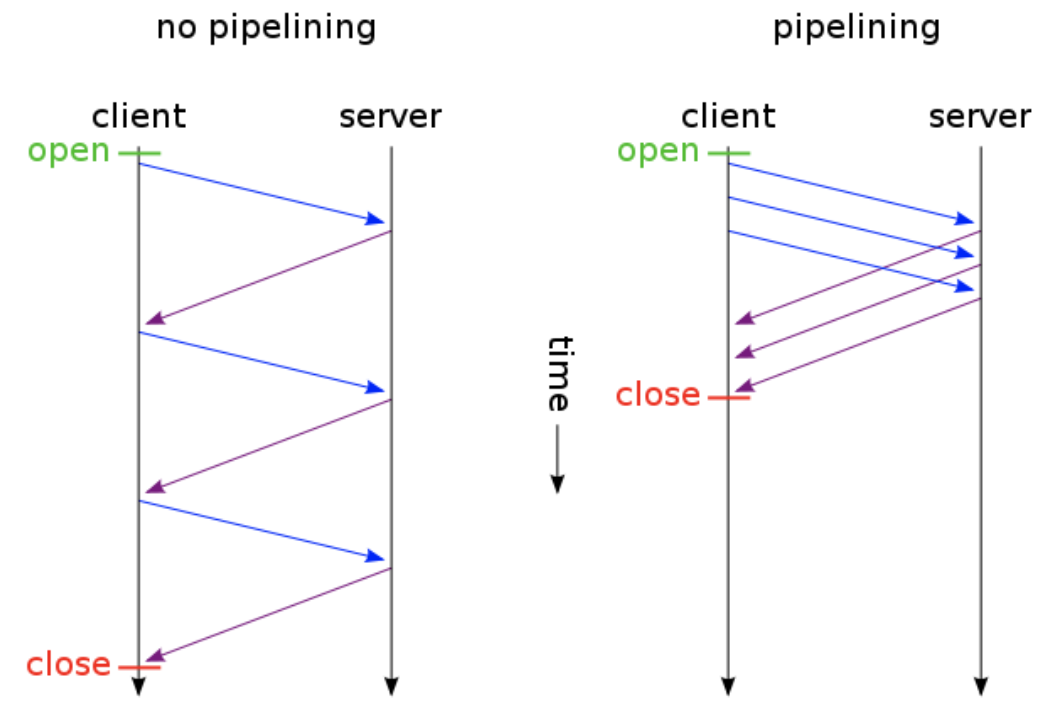
\includegraphics[width=0.6\linewidth]{res/pipelining.png}
\end{figure}
Un messaggio HTTP è formato da request/status line, header, body. Una request line è composta da \code{metodo target versioneHTTP}. Una status line è \code{versioneHTTP statusCode reasonPhrase}. Gli headers sono in formato MIME e specificano i metadati della richiesta come data, versione MIME, encoding, connessione, proxy/gateway, content-type, content-length, encoding, linguaggio, scadenza, data di modifica\dots Termina sempre con un carriage return (\code{\\r\\n}). 
\subsubsection{Metodi HTTP}
Prima di elencare i metodi, denotiamo due caratteristiche:
\begin{itemize}
    \item \textbf{Idempotenza}: significa che il metodo, chiamato più volte, restituirà sempre lo stesso risultato.
    \item \textbf{Safety}: significa che il metodo non modifica le risorse.
\end{itemize}
Procediamo elencando i metodi:
\begin{itemize}
    \item \textbf{GET}: \textit{safe ed idempotente.} Utilizzato per richiedere una risorsa, ottenuta nella risposta.
    \item \textbf{POST}: \textit{non safe, non idempotente.} Utilizzato per creare/aggiornare una risorsa. Chiamato ripetutamente, creerà più volte la risorsa.
    \item \textbf{PUT}: \textit{idempotente ma non safe.} Utilizzato per creare/aggiornare una risorsa.
    \item \textbf{DELETE}: \textit{idempotente ma non safe.} Elimina la risorsa specificata.
    \item \textbf{HEAD}: \textit{safe ed idempotente.} Come una GET ma restituisce solo l'header del messaggio.
\end{itemize}
Prima di procedere, distinguiamo le differenze tra POST e PUT: nella creazione di risorse, POST non specifica l'ID, mentre PUT si. Nell'update, POST permette di inviare la risorsa parzialmente (solo la parte da updatare), mentre PUT richiede la risorsa completa.
\subsubsection{Header delle richieste HTTP}
L'header contiene varie informazioni:
\begin{itemize}
    \item User-Agent: descrive il client che ha originato la richiesta
    \item Referer: URL della pagina che ha generato la richiesta 
    \item Host: dominio e porta a cui viene eseguita la richiesta
    \item From: indirizzo email del requester 
    \item Range: range della richiesta (utilizzato per riprendere i download)
    \item Accept, Accept-Charset, Accept-Encoding, Accept-Language: si spiega da solo; il client specifica cosa può accettare, il server decide il suo preferito
    \item If-Modified-Since, If-Unmodified-Since: permette di creare GET condizionali, ad esempio se ho una risorsa in cache e voglio verificare che sia aggiornata
    \item Authorization, Proxy Authorization 
\end{itemize}
\subsubsection{Messaggi di risposta HTTP}
La status line contiene un codice di stato:
\begin{itemize}
    \item 1xx - Informational: temporaneo mentre la richiesta viene eseguita
    \item 2xx - Successo: richiesta eseguita 
    \item 3xx - Redirection: il server ha ricevuto la richiesta ma sono necessarie altre azioni del client 
    \item 4xx - Client error: la richiesta è sbagliata
    \item 5xx - Server error: il server non è riuscito ad eseguire la richiesta 
\end{itemize}
Nell'header troviamo:
\begin{itemize}
    \item Server: stringa che descrive il server 
    \item WWW-Authenticate: contiene una challenge per il client; in caso di 401 unauthorized, il client utilizzerà la challenge per generare un codice di autorizzazione.
    \item Accept-Ranges: specifica il tipo di ranges accettabili (bytes/nulla)
\end{itemize}
\subsubsection{Cookies}
Molti siti utilizzano i cookies. Essi sono composti da 4 componenti: header line della prima risposta HTTP, header line nella prossima richiesta HTTP, file sull'host, DB sul backend del sito. 
\subsubsection{Proxy}
Il proxy è un'applicazione intermediaria che ha funzionalità server e client. Un \textbf{transparent proxy} non modifica la richiesta o risposta (es. HTTP tunneling), un \textbf{non-transparent proxy} modifica la richiesta/risposta per fornire servizi aggiuntivi.
Possiamo utilizzare un proxy server per soddisfare richieste senza coinvolgere il server originale: se la richiesta è nella cache, restituisce la risposta, altrimenti la inoltra. 
\subsection{Apache}
\textbf{Apache} nasce dal desiderio di migliorare httpd, il software server più utilizzato agli inizi di internet; è attualmente utilizzato per mantenere più del 50\% di internet. La sua architettura
 è formata da: 
 \begin{itemize}
     \item Moduli: compilati staticamente nel server o contenuti in una directory /modules o /libexec, caricata dinamicamente a runtime
    \item Apache httpd: implementa il ciclo di processamento delle richieste, composto da più fasi
    \item Multi-Processing Module: strato intermedio tra Apache e il sistema operativo, che gestisce i thread/processi
    \item Apache Portable Runtime: librerie che forniscono uno strato tra il sistema operativo e le utilities, in modo da poter essere portable
    \end{itemize}
Apache 2.0 utilizza un processo per connessione, I/O blocking. I Multi-Processing Modules bindano le porte della macchina e accettano richieste. 
\subsubsection{Configurazione}
La configurazione è eseguita tramite semplici file di testo, posizionati in varie directory e spesso divisi in più file e caricati tramite \textit{Include directives}. Una configurazione minimale richiede 5 directives:
\begin{enumerate}
    \item \code{User}: setta lo user ID con cui il server risponderà a richieste (utilizzare i permessi minimi)
    \item \code{Group}: setta il gruppo con cui il server risponderà a richieste (necessario avviare il server come root inizialmente)
    \item \code{ServerName}: setta lo schema delle richieste, hostname e porta. È in pratica l'URI.
    \item \code{DocumentRoot}: setta la directory di base delle richieste, a meno di specifiche di \textit{Alias.}
    \item \code{Listen}: setta la/le porta/e su cui accettare richieste
\end{enumerate}
In più, abbiamo:
\begin{itemize}
    \item \code{ErrorLog}: indica dove salvare il log degli errori
    \item \code{CustomLog}: indica un file dove salvare un log delle richieste, ed un filtro per decidere quali richieste loggare.
    \item \code{Include}: permette di includere altri file di configurazione
    \item \code{LoadModule}: linka una libreria/file oggetto e lo aggiunge ai moduli attivi.
    \item \code{IfModule}: permette di verificare se un modulo è installato ed eseguire directives di conseguenza.
\end{itemize}
Tramite virtual hosting possiamo hostare più siti sullo stesso server, distinguendoli in due possibili modi: tramite IP o nome. Con la seconda, non c'è necessità di IP multipli. 
Possiamo anche applicare delle configurazioni locali in determinate directory, e tramite le Options directives attivare/disattivare features, come: ExecCGI, FollowSymLinks, SymLinksIfOwnerMatch, Includes, IncludesNOEXEC, Indexes.
Inoltre, è possibile utilizzare i file \code{.htaccess} per definire cambiamenti alla configurazione in directories: inseriamo il file in una cartella e tutte le modifiche alla configurazione verranno eseguite lì e nelle subfolders. Tramite la \code{AllowOverride} della configurazione, decidiamo quali directives possono essere overridate dagli htaccess. Per migliorare le performance di Apache, il sistemosta può modificare le opzioni di Apache: è però sconsigliabile usare spazio di swap (RAM virtuale). Infine, con la directive \code{ErrorDocument}, specifichiamo cosa fare quando si incorre in un errore HTTP specifico, con 4 possibilità: messaggio hardcoded di errore (default), messaggio custom, redirect interno, redirect esterno.
\subsubsection{Avvio di Apache}
Su \href{https://www.youtube.com/watch?v=dFUlAQZB9Ng}{sistemi Unix} httpd viene eseguito come daemon continuamente; se la directive Listen è sulla porta 80, è necessario avviare Apache come root perché è una porta speciale (poi verranno lanciati child processes). Lanciamo Apache con l'\code{apachectl} control script, che setta le variabili ENV necessarie e poi avvia httpd. Se l'avvio è succesful, il server viene detacchato dalla console (scusate). Si può usare apachectl per terminare Apache, o killare il daemon.
\subsection{HTML}
Il web è basato su tre risorse: gli URI, i protocolli, e HTML. \textbf{HTML} è un linguaggio universale che permette la creazione di documenti con formattazioni, contenuti, link, design. Nasce dalla mente di Tim Berners-Lee e conta attualmente 5 versioni major, la cui ultima è 5.2. Per promuovere l'interoperabilità, ogni documento HTML deve specificare il suo character set, formato da repertorio e code positions. Inoltre, va specificato l'encoding nell'header delle richieste HTTP. Distinguiamo tra 3 parti: una linea di versione HTML, un header, un corpo. Nell'header possiamo trovare varie tipologie di tag: \code{TITLE}, \code{BASE}, \code{LINK}, \code{SCRIPT}, \code{STYLE}, \code{META}. Nel corpo, possiamo trovare DIV (block-level) e SPAN (inline). Un heading descrive l'argomento della sezione che introduce (H1..H6 in base all'importanza). Abbiamo anche alcuni tag per il testo: \code{BR} va a capo, \code{P} delimita un paragrafo, \code{PRE} delimita un testo preformattato, \code{EM}, \code{STRONG}, \code{CITE}, \code{DFN}, \code{CODE}, \code{SAMP}, \code{KBD}, \code{VAR}, \code{ABBR}, \code{ACRONYM}, \code{BLOCKQUOTE}, \code{Q}, \code{SUB}, \code{SUP}. Possiamo creare liste: \code{UL} (\textit{Unordered List}), \code{OL}(\textit{Ordered List}), \code{DL}(\textit{Definition List}). Possiamo creare tabelle: \code{TABLE, TR, TD}. Possiamo spaziarle utilizzando \code{rowspan} e \code{colspan}, captionarle con \code{CAPTION}. Possiamo creare links con il tag \code{A}, avente attributi \code{href} e \code{target}(\_blank, \_self, \_parent, \_top). Dando ID agli elementi HTML possiamo cercarli tramite gli anchor link (\#riferimento). Con l'elemento \code{IMG} embeddiamo immagini definite nell'attributo \code{src}. Con \code{OBJECT} definiamo oggetti come risorse, applets, plugin. Con i frame possiamo generare views multiple; un frame ha head, frameset e body, con attributi rows e cols. Possiamo anche creare forms, che contengono contenuto, markup, controlli, labels e li inviano ad un'action (tramite GET o POST). In HTML5 sono stati inoltre definiti nuovi tag, semantici (header, footer, article, section) , di controllo (numeri, date, orari, calendari, range), grafici (svg, canvas), multimediali (audio, video). Non sono più supportati i frames, sostituiti dagli iframes.
\subsection{CSS}
HTML non è nato per contenere tag di definizione di stile, ma piuttosto per mostrare dati. Quando cominciarono a venire aggiunti tag di stile ad HTML 3.2, come \code{font}, \code{color}, si capì che non poteva funzionare. Il World Wide Web Consortium (W3C) creò quindi \textbf{Cascading File Sheets} (CSS). In HTML4, tutta la formattazione poté quindi essere definita separatamente dall'HTML, dando la possibilità di modificare l'intero sito con un solo sito web. 
\subsubsection{Sintassi}
La sintassi consiste in un selettore, seguito da varie dichiarazioni:
\begin{center}
    \code{h1 \textbraceleft}
    \code{color:blue;}
    \code{font-size:12px;}
    \code{\textbraceright}
\end{center}
Il selector punta all'elemento HTML desiderato, mentre nel blocco di dichiarazione inseriamo una o più dichiarazioni separate da ;.
I selettori possono indicare una tipologia HTML, come \code{p}, una classe, come \code{.rowDiv}, un ID, come \code{\#title}. Possiamo includere CSS in tre modi:
\begin{itemize}
    \item Style sheet esterno: \code{<LINK rel="stylesheet" type="text/css" href="file.css">}
    \item Style sheet interno: \code{<STYLE> body\textbraceleft\textbraceright</STYLE>}
    \item Inline: \code{<H1 style="color:blue;">}
\end{itemize}
\subsubsection{Attributi notevoli}
Alcuni attributi importanti:
\begin{itemize}
    \item \textbf{Background}: background-color, background-image, background-repeat, background-attachment, background-position
    \item \textbf{Text}: color, text-align, text-decoration, text-transform, text-indent
    \item \textbf{Fonts}: permette di definire una font family (generica o specifica) con sistema fallback: le prova in ordine finché non trova la funzionante; è quindi meglio partire con specifica e terminare con generica. Oltre a font-family, abbiamo font-style (italic, oblique), font-size, font-weight
    \item \textbf{Links}: possiamo applicare ogni CSS property, ed in più abbiamo 4 selector speciali (A:link, A:visited, A:hover, A:active)
    \item \textbf{Lists}: possiamo settare i marker delle liste, o addirittura immagini come item markers con list-style-image 
    \item \textbf{Tables}: possiamo specificare i borders tramite la proprietà border, e anche width/height. Inoltre, anche text-align e vertical-align sono disponibili.
\end{itemize}

\subsubsection{Box model}
In CSS sfruttiamo il \textit{pattern} del box model: essenzialmente è ciò che wrappa un contenuto, che ci permette di aggiungere padding, bordi, margini. 
\begin{figure}[H]
    \centering
    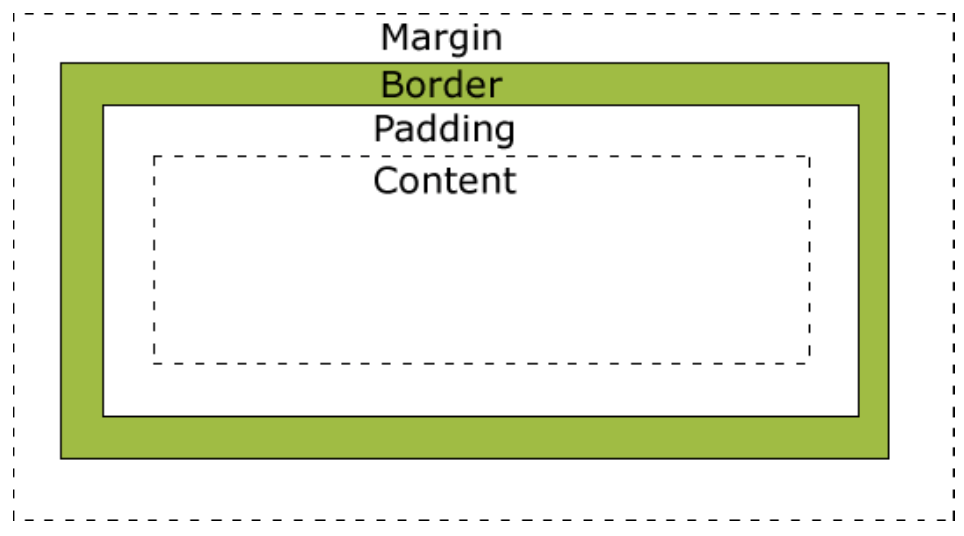
\includegraphics[width=0.6\linewidth]{res/boxmodel.png}
\end{figure}
\subsection{XML}
Sembrerà un linguaggio inutile e passato (perché lo è), ma nella sezione SOA ci sono ben due lezioni che si basano su sto schifo. \textit{Ocio.} XML sta per \textbf{eXtensible Markup Language} e serve per trasportare informazioni, non per presentarli (come HTML). I tag non sono definiti in uno standard, ma dall'utente. Possiamo, per esempio sfruttare XML per separare i dati variabili da HTML. 
\paragraph{Quando usare XML?} XML semplifica il salvataggio e la condivisione di dati, essendo un formato standard basato su testo. Semplifica i cambiamenti di piattagorma, essendo testo semplice. Tra i linguaggi scritti in XML, citiamo SVG, WSDL, RSS.
\subsubsection{Struttura}
Il documento XML inizia con il prologo, che definisce la versione XML. Comincia poi l'albero, che ha una root e delle leaves. I figli sullo stesso livello sono detti siblings (fratelli). Tutti i figli possono avere un contenuto e degli attributi. In XML è illegale omettere il tag di chiusura (tranne ovviamente nel prologo). I tag XML sono \textbf{case sensitive}. Gli attributi devono essere sempre tra virgolette. I commenti sono come in HTML: \code{<!-- Commentino -->}. XML non tronca gli spazi bianchi come HTML, e salva le nuove linee come \code{LF}. Bisogna stare attenti ad alcuni caratteri, come $<$, che vanno escapati con sequenze specifiche: \&gt;, \&amp, \&apos, \&quot;. Gli elementi XML devono seguire alcune regole di nomenclatura:
\begin{itemize}
    \item Case sensitivity
    \item Inizio con lettera o underscore
    \item Non si può iniziare con "XML"
    \item Possono contenere lettere, numeri, trattini, underscore, punti
    \item Non possono contenere spazi 
    \item Le lettere accentate non sono un problema (ma occhio ai software)
\end{itemize}
Gli attributi solitamente forniscono informazioni che non sono parte dei dati, ad esempio, se avessimo un contenuto file, l'attributo potrebbe essere il filetype. Alcuni problemi degli attributi:
\begin{itemize}
    \item Non possono contenere valori multipli
    \item Non possono contenere alberi 
    \item Non sono facilmente espansibili
\end{itemize}
Per evitare conflitti di nomi, possiamo utilizzare dei prefissi di namespace con l'attributo xmlns:
\begin{verbatim}
<h:table xmlns:h="http://www.w3.org/TR/html4/"> 
    <h:tr>
        <h:td>Apples</h:td>
        <h:td>Bananas</h:td>
    </h:tr>
</h:table>
\end{verbatim}
Dopo aver definito un namespace, tutti i contenuti con quel prefisso verranno collegati al namespace. Definire un namespace di default è utile: ci evita di utilizzare prefissi in tutti i children. 
Possiamo utilizzare anche caratteri internazionali: è però importante specificare l'encoding nel prolog. 
\subsubsection{Validità e document types}
Un documento XML corretto è detto \textit{ben formato}. Un documento XML valido deve essere compatibile ad una \textbf{document type definition}. Ne abbiamo due diverse: DTD (\textit{Document Type Definition}) e XML Schema (\textit{basata su XML}). Usiamo questi document type per vari scopi: decidere standard, verificare dati dall'esterno, verificare dati nostri. XML non lo richiede per forza, ma in ambienti di produzione ci vuole. Lo scopo di un DTD è definire la struttura, con una lista di elementi validi. Possiamo anche usarlo per definire caratteri speciali e stringhe di caratteri. L'\textbf{XML Schema} è un'alternativa basata su XML a DTD.

\subsection{JSON}
\textit{Finalmente.} JSON è il cugino che ce l'ha fatta di XML. Sta per \textbf{JavaScript Object Notation}, ed è come XML una sintassi per salvare e scambiare dati, più leggera e semplice di XML. Dal momento che JSON è proprio il modo di definire oggetti in JavaScript, non necessita di parser. Similarità con XML: self-describing, gerarchico, portable, fetchabile con una XMLHttpRequest. Differenze con XML: niente tag di chiusura, più breve, più veloce, presenza di arrays. La sintassi di JSON è derivata da JS: i dati sono accoppiati nome/valore, separati da virgole, oggetti delimitati da \textbraceleft\textbraceright, arrays delimitati da $[]$. Un valore JSON può essere un numero, stringa, boolean, array, oggetto, null.
\subsection{Search Engines}
L'\textbf{information retrieval} è parte della computer science che studia il recupero di informazioni da una collezione di documenti, soddisfando le necessità dell'utente, solitamente definite in linguaggio naturale. 
La \textbf{web search} è molto simile, con alcune differenze: links tra web pages, collezionare documenti è molto più difficile, il numero di utenti è grande, lo spam è un problema. La struttura di un web search engine è composta da un downloader, un crawler, un indexer\dots Abbiamo eterogeneità multiple: utenti, linguaggi, document types, queries (informational, navigational, transactional, connectivity). Un crawler feeda continuamente l'indexer con informazioni nuove o aggiornate. Distinguiamo inoltre tra surface web, indexato, e deep web (da non confondere con darkweb) ossia la parte di internet non indexata, composta da pagine dinamiche, contenuti privati, script, formati particolari. 
\subsubsection{Web Graph}
Possiamo vedere le pagine, linkate tra loro, come un grafico di pagine collegate tra in-links e out-links. La distribuzione dei links non è randomica ma segue una \textit{power law}: il numero di pagine con k \textit{in-links} è proporzionale a $k^{-2.1}$. Alcuni studi hanno mostrato che il web graph ha \textit{bowtie shape}. 
Un crawler consiste in una queue di URI da visitare, un metodo per ottenere i dati, un parser che estragga i link, una connessione all'indexer. Il crawler dev'essere highly scalable: abbiamo 60mld di pagine sul web. Dobbiamo inoltre tenere conto di altri problemi: spam, duplicati, spider traps, distribuzione, latenza, banda, profondità, desideri dell'owner. In quanto owner possiamo escludere alcune risorse dall'accesso dei robots, tramite il file robots.txt. Per l'indexing, sfruttiamo la link analysis: i link sono raccomandazioni, gli anchor texts descrizioni del documento. 
\subsubsection{PageRank}
PageRank è l'algoritmo di Larry Page (il signor Google) sviluppato a Stanford. È un algoritmo di link analysis che produce un ranking non dipendente dalle queries. È eseguito periodicamente dall'indexer. L'algoritmo si basa sulla probabilità che un utente random clicki su un link che porti alla pagina da un'altra, calcolata ricorsivamente sulla probabilità della pagina attuale e via andare\dots PageRank è usato ancora oggi (in parte), soprattutto in formato topic-sensitive: una pagina su un topic specifico può non essere utile globalmente ma essere importante per il topic stesso. 
\subsubsection{HITS}
HITS è un altro algoritmo. Cominciamo col distinguere due tipi di pagine web: authorities (fonti autoritarie sull'argomento), hubs (puntatori all'authority). C'è una relazione di reinforcement: hub di qualità puntano ad authorities di qualità. Seguiamo due fasi:
\begin{enumerate}
    \item \textbf{Sampling phase}: le parole della query vanno a costruire un root set di pagine, che viene espanso a un base set, aggiungendo tutte le pagine linkate dal root set
    \item \textbf{Weight-propagation phase}: ogni pagina riceve un authority-weight $a_p$ e un hub-weight $h_p$ pari a 1. A questo punto, $a_p$ è la somma degli hub weights che puntano alla pagina, mentre $h_p$ è la somma degli authority weights delle pagine linkate da p. Poi, applichiamo una normalizzazione finché i weights non convergono. 
\end{enumerate} 
A volte HITS tende a generalizzare o a deviare dal topic, soprattutto quando gli hubs coprono più topic; una soluzione potrebbe essere comparare le parole della query con quelle che circondano il link, o frammentare un grande hub in hublets minori, ed ignorare quelli unrelated. 
\subsubsection{HITS vs PageRank}
PageRank può essere precomputed, mentre HITS deve essere computato a query time. Abbiamo poi scelte diverse riguardanti il modello formale.

\section{JavaScript}
\subsection{Basics}
JavaScript è il linguaggio di programmazione che permette di programmare il comportamento delle pagine web. Seguendo il pattern MVC, abbiamo che il model è gestito da XML/JSON, la view da HTML+CSS , il controller da JavaScript. JavaScript non è Java e non è un linguaggio di scripting. ECMAScript è la standardizzazione ufficiale del linguaggio. Il core di JS definisce un'API minimale, ma è l'environment ad avere le responsabilità maggiori: il browser, Rhino o Node. 
Possiamo embeddare JS in HTML tramite: inline (tag \code{<script>}), esterno (sempre tag \code{<script>} con \code{src}), in un event handler come l'onclick, in un URL che utilizza il protocollo \code{javascript:}. Una filosofia detta \textbf{unobstrusive JavaScript} sottolinea che contenuto (HTML) e comportamento (JS) devono essere il più separati possibile. JS non ha metodi di print definiti, ma usiamo \code{window.alert()}, \code{document.write()}, \code{innerHTML}, \code{console.log()}. Gli statement sono separati da ;, e composti da valori, operatori, espressioni, keywords, commenti. Definiamo tra valori fissi (\textbf{literals}) e variabili (\textbf{variables}). Utilizziamo la keyword \code{var} per definire variabili, che in JS sono \textbf{untyped}. Essendo untyped abbiamo possibilità di confusione; JS interpreta le operazioni da sinistra a destra. 
\begin{figure}[H]
    \centering
    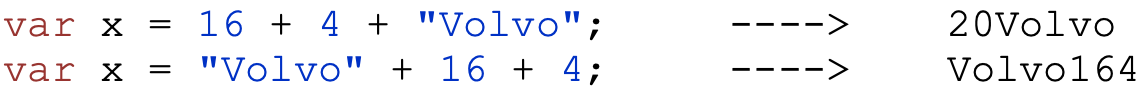
\includegraphics[width=0.4\linewidth]{res/JSconfusion.png}
\end{figure}
Abbiamo i soliti operatori; la concatenazione di stringhe è fatta con \code{+}. Esiste l'operatore condizionale \code{ ? : }. I commenti sono fatti con \code{//} e \code{/* */}. Gli identifiers possono iniziare con lettere, underscore o dollaro e contenere lettere, numeri, underscores, dollari. Gli identifiers sono case sensitive. Le funzioni sono definite dalla keyword \code{function} seguita da nome e argomenti. Le variabili possono anche contenere oggetti, definiti con la forma classica di JS. Inoltre, gli oggetti possono contenere funzioni (questo è importante) come se fossero semplici attributi. Possiamo creare oggetti in tre modi: con l'object literal (come JSON), con la keyword new \code{Object ()} e poi settando attributi, o con una funzione costruttrice. Gli oggetti creati con i primi due metodi ereditano da un prototipo detto \code{Object.prototype}, che è in cima alla scala gerarchica. JS ha costruttori per gli oggetti nativi, come Object, String, Number, Boolean, Array, RegExp, Function e Date, ma è meglio utilizzare i literals, come \textbraceleft\textbraceright, "", 0, false, $[]$, $/()/$, function$(){};$. Gli oggetti sono indirizzati per reference, non valore, quindi la copia non è fattibile con $=$. Possiamo aggiungere attributi ad un oggetto semplicemente assegnandoli, ed eliminarli con la keyword \code{delete}. Tramite la proprietà prototype, possiamo modificare prototipi già definiti. 
\begin{figure}[H]
    \centering
    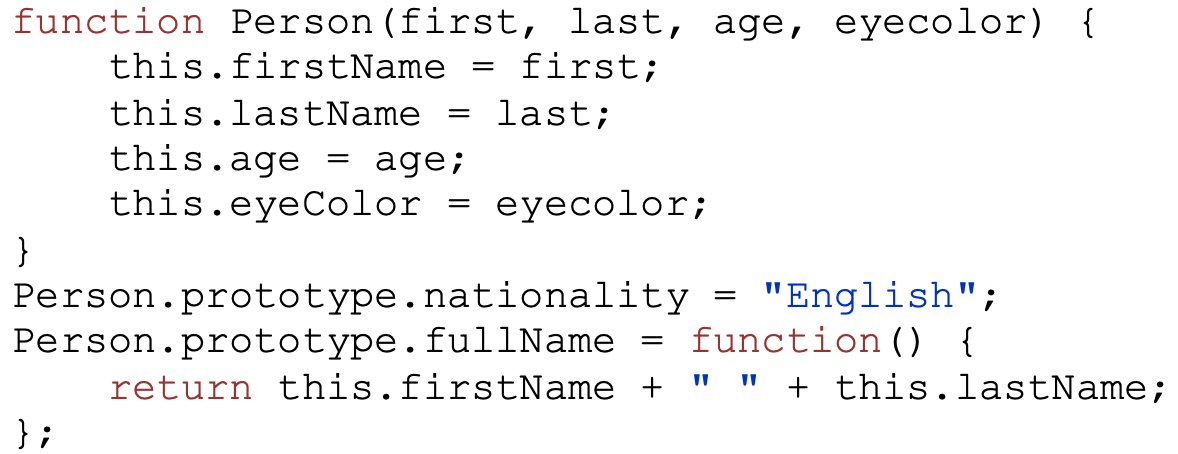
\includegraphics[width=0.4\linewidth]{res/prototype.png}
\end{figure}
Possiamo loopare tra tutte le proprietà di un oggetto usando \code{for..in}.
La sintassi \code{with (object)${}$} utilizza object come prefisso di tutti gli statement enclosati. Con ECMAScript6 sono state introdotte le classi OOP, con eredità. Gli arrays sono oggetti speciali con indici numerici e non testuali, che hanno dei metodi built-in comodi come \code{length}, \code{sort()}, \code{pop()}, \code{push()}. La sort lavora però su stringhe, quindi ad esempio 25 è più grande di 100. Possiamo però fornire come argomento una compare function. 
\subsection{Client-side JS}
L'oggetto window è l'entry point principale di tutte le feature di JS client-side. JavaScript è più puntato sulle web applications che sui web documents: i secondi funzionano con JS disattivato, le prime no. Quando un HTML parser incontra uno script, lo esegue di default. Solo gli script sincroni possono usare \code{document.write()} per inserire testo nell'input stream. Il tag script può avere attributi \code{defer} e \code{async}: il primo lo esegue a fine caricamento, il secondo lo esegue al più presto ma senza bloccare il parsing. Il core di JS non contiene meccanismi di threading, quindi due event handlers non gireranno mai allo stesso tempo; l'esecuzione single-threaded significa che i browser devono smettere di rispondere agli input quando gli script vengono eseguiti. Se c'è molta computazione, sarebbe meglio lasciar caricare il documento prima. Questa la timeline degli eventi:
\begin{enumerate}
    \item Il browser crea un oggetto document e comincia a parsare la web page, aggiungendo gli elementi e i text nodes. \code{document.readyState} è ora "loading"
    \item Quando l'HTML parser incontra degli elementi \code{<script>} senza async o defer, li aggiunge al documento e li esegue. 
    \item Quando l'HTML parser incontra degli script async comincia a scaricare lo script e continua a parsare. Lo script verrà eseguito appena scaricato.
    \item Quando il documento è parsato, \code{document.readyState} è "interactive"
    \item Ogni script con l'attributo defer viene eseguito nell'ordine di lettura. Questi hanno accesso alla document tree e non devono usare \code{document.write()}. 
    \item Il browser lancia un evento \code{DOMContentLoaded} sull'oggetto document. Questo segna la transizione dalla fase sincrona di esecuzione alla fase asincrona event-driven. 
    \item Il documento è parsed, ma potrebbero ancora mancare risorse come le immagini. Quando è tutto pronto, \code{document.readyState} passa a "complete"
\end{enumerate}
JS non fornisce alcun metodo per scrivere o eliminare file sul computer, ma può ottenere un FileSystem privato. 
\subsubsection{Same Origin Policy}
La same origin policy indica che uno script può leggere solo le proprietà di finestre e documenti che hanno la stessa origine (protocollo, host, porta) del documento che contiene lo script. La policy è applicata alle richieste HTTP fatte con l'oggetto XMLHttpRequest, che permette al JS client-side di fare richieste HTTP al server da dove ha caricato il documento, ma non ad altri server. Per richieste cross-origin bisogna attivare \textit{Cross-Origin Resource Sharing}. 
\subsubsection{L'oggetto window}
L'oggetto \textbf{window} è l'oggetto globale per il client-side JS, le cui proprietà sono collegate a timers, location/navigation, history, browser informations, dialogs, document elements, comunicazione cross-window. 
\paragraph{Timers} I \textbf{timers} vengono settati con \code{setTimeout} che esegue una funzione dopo un numero definito di ms, e \code{setInterval}, che fa la stessa cosa ciclicamente ad intervalli.
\paragraph{Location e navigation} La proprietà \code{location} dell'oggetto window si riferisce ad un oggetto location, che rappresenta l'URL corrente e i metodi per far caricare alla window un nuovo documento. La proprietà \code{href} dell'oggetto location è una stringa contenente l'URL, altre proprietà sono protocol, host, hostname, port. pathname, search, hash. L'hash ritorna l'anchor link, mentre search le query delimitate da ?. Il metodo assign della location carica un nuovo URL, replace lo fa rimuovendo la pagina corrente dall'history, reload aggiorna. 
\paragraph{History} La proprietà \code{history} della window contiene la cronologia. Ha proprietà length, metodi \code{back()} e \code{forward()}, \code{go(n)} che va avanti o indietro di n passi
\paragraph{Navigator} La proprietà \code{navigator} contiene informazioni sul browser. L'utilizzo di queste informazioni è sconsigliato: è meglio utilizzare il feature testing. Tra le proprietà citiamo appName, appVersion, userAgent, platform. Abbiamo poi alcune proprietà non-standard: onLine, geolocation, javaEnabled(), cookieEnabled.
\paragraph{Screen} La proprietà \code{screen} fornisce informazioni sulle dimensioni e colori del display: width, height, availWidth, availHeight (escludono menubar ecc.), colorDepth. 
\paragraph{Dialogs} L'oggetto window fornisce tre metodi per generare dialogs: alert(), confirm(), prompt().
\paragraph{Elementi HTML} Ogni elemento del documento HTML che hanno un id diventano proprietà di window, contenenti l'oggetto HTMLElement. È però raccomandato utilizzare \code{document.getElementById()}. 
\paragraph{Multiple windows} La comunicazione tra windows è possibile solo tra finestre same-origin. Il metodo \code{open()} apre una nuova finestra e ritorna l'oggetto relativo, prendendo 4 argomenti: URL, nome, attributi size/feature, boolean che indica se creare un nuovo record nell'history. Il metodo \code{close()} chiude la finestra indicata. Possiamo anche accedere agli oggetti window degli iframe tramite \code{iframe.contentWindow} e al document tramite \code{iframe.contentDocument}. 
\subsubsection{Scripting di documenti}
Il DOM, \textbf{Document Object Model} è lo standard W3C per accedere ai documenti, separato in Core, XML, HTML. Quest'ultimo è uno standard e interfaccia di programmazione per HTML, definendo: gli elementi HTML come elementi, le proprietà, i metodi, gli eventi. Insomma: \textbf{l'HTML DOM è uno standard per come ottenere, modificare, aggiungere o eliminare elementi HTML.}
Per ottenere un elemento HTML il modo più semplice è usare \code{document.getElementById()}, per il contenuto poi usiamo \code{innerHTML}. Possiamo, inoltre, modificare gli attributi con \code{element.attribute}, e lo stile \code{element.style.property}. Possiamo aggiungere/rimuovere elementi al documento con \code{document.createElement()}, \code{document.removeChild()}, \code{document.appendChild()}, \code{document.replaceChild()}, \code{document.write(text)}, o settare event handlers con \code{document.getElementById(id).onclick = function $(){}$}. Altri modi di ottenere elementi sono getElementsByTagName e getElementsByClass, che ritornano liste (non array: sono navigabili allo stesso modo ma mancano alcuni metodi). L'HTML DOM ha una struttura ad albero, in cui gli elementi HTML sono nodi, aventi attributi \code{nodeName}, \code{nodeValue}, \code{nodeType}.
\subsection{Client side - AJAX}
Gli eventi HTML sono cose che accadono agli elementi HTML, a cui JS può reagire. Gli elementi HTML possono avere un attributo onclick a cui associare una funzione JS. Oltre ad onclick, abbiamo: onchange, onmouseover, onmouseout, onkeydown, onload\dots Gli event handler possono essere utilizzati per gestire gli input utente. L'HTML DOM permette di assegnare event handler agli elementi HTML. 
\paragraph{onload e onunload} Vengono triggerati quando l'utente entra o lascia la pagina, sono utilizzabili per controllare il browser, o gestire i cookies.
\paragraph{onchange} Utilizzato spesso per la validazione dei field.
\paragraph{onmouseover e onmouseout} Triggerano una funzione quando l'utente sposta il mouse sull'elemento. 
\paragraph{onmousedown, onmouseup, onclick} Si spiegano da soli: il primo è il down, poi up, infine click. 

Utilizziamo il metodo \code{element.addEventListener(event, function, useCapture)} per aggiungere un event listener. Distinguiamo tra bubbling (primo trigger è il più interno) e capturing (primo trigger è il contenitore) come metodi di trigger. Utilizzando \code{addEventListener} possiamo aggiungere più event handlers a uno stesso evento. 
\subsubsection{AJAX}
AJAX significa \textbf{Asynchronous JavaScript and XML}, ed è una tecnica per creare pagine web veloci e dinamiche. AJAX permette di aggiornare le webpages in modo asincrono, scambiando dati con il server e modificando il contenuto senza ricaricare tutta la pagina. Il punto chiave di AJAX è l'oggetto \code{XMLHttpRequest}, che permette di fare richieste HTTP. Bisogna verificare se è supportato, altrimenti usare un ActiveXObject (\textit{Microsoft vaffanculo}). Apriamo la richiesta tramite \code{open(method, url, async)} e la inviamo tramite \code{send()} per GET e \code{send(string)} per POST. Per evitare di farci ritornare dati cachati, aggiungiamo alla GET una query casuale. Per aggiungere headers a una POST, utilizziamo \code{setRequestHeader(header, value)}. Bisogna stare attenti alla same-origin policy. Per ottenere la risposta, utilizziamo l'attributo \code{responseText} o \code{responseXML} dell'oggetto richiesta. Come il document, la request ha un attributo \code{readyState} (0..4), un relativo evento \code{onreadystatechange} e un attributo status che contiene lo status HTTP. Quando readyState è 4 e status 200, è andato tutto bene. Potremmo quindi aggiungere una callback all'onreadystatechange, verificando queste due condizioni prima.

\subsubsection{jQuery}
\textbf{jQuery} è una leggera libreria "\textit{write less, do more}" che rende più semplice il JS. Abbiamo due versioni, una di produzione minified, difficilmente leggibile, e una di sviluppo. Per utilizzare jQuery lo referenziamo nell'head del documento, hostandolo sul server o caricandolo da un CDN. La sintassi di jQuery permette di selezionare elementi HTML semplicemente: \$$($selettore$)$. Per evitare di eseguire codice jQuery prima del corretto caricamento della pagina, mettiamo il codice dentro un document ready event. In jQuery, la maggior parte dei DOM events hanno un metodo jQuery corrispondente, per esempio \code{\$("p").click(function$(){}$)}. jQuery permette anche di definire eventi custom, firabili con \code{trigger(nome, datiOpzionali)}, e handlabili con \code{.on("evento", function$(){}$)}. 
\subsubsection{Animazioni con jQuery}
jQuery permette anche di implementare animazioni: un esempio sono i metodi \code{hide(speed, callback)} e \code{show(speed, callback)}. Speed può essere "slow", "fast", o un valore di millisecondi. Callback viene invece eseguito al termine dell'animazione. Il metodo \code{toggle()} alterna tra show e hide. Abbiamo anche dei metodi di fade: \code{fadeIn(s, c)}, \code{fadeOut(s, c)}, \code{fadeToggle(s, c)}, \code{fadeTo(s, opacity, callback)}. Possiamo anche slidare elementi: \code{slideDown(s, c)}, \code{slideUp(s, c)}, \code{slideToggle(s, c)}. Grazie al metodo \code{animate(\textbraceleft parametri\textbraceright, s, c)} possiamo creare animazioni custom modificando proprietà CSS. Di default, jQuery lavora per queue sulle animazioni: le fa una alla volta.
\subsubsection{Manipolazione del DOM con jQuery}
jQuery permette anche di \textbf{manipolare il DOM} tramite 4 metodi che settano o leggono: \code{text()}, \code{html()}, \code{val()}, \code{attr()}. Abbiamo metodi per aggiungere contenuto: \code{append()}, \code{prepend()}, \code{after()}, \code{before()}. Metodi per rimuovere contenuto: \code{remove()} (filtrabile), \code{empty()}. Possiamo modificare il css: \code{addClass()}, \code{removeClass()}, \code{toggleClass()}, \code{css()}. Questo non è tutto: ci sono anche metodi per modificare dimensioni, navigare gli elementi, funzionalità AJAX (ad esempio, richieste GET con \code{\$.get(url, callback))}.
\subsubsection{Client-side storage}
Le web apps possono utilizzare API del browser per salvare dati sul computer. I dati salvati possono essere visualizzati solo da pagine dello stesso sito. Abbiamo più modi di salvare roba: WebStorage API, Cookies, Filesystem API\dots
\paragraph{Web Storage} L'API Web Storage fornisce due oggetti: \code{window.localStorage} (senza scadenza) e \code{window.sessionStorage} (eliminata con la chiusura della tab). Prima di utilizzarle è bene verificare la disponibilità della feature. 
\subsubsection{Scripted graphics}
Generare grafiche complesse nel browser è molto meglio: rimuove il carico dal server per affidarlo al computer, risparmiando in banda, CPU, RAM\dots Inoltre è consistent con le moderne architetture applicative. In HTML5 è stato introdotto l'elemento \code{<canvas>} che ha lo scopo di ospitare grafiche generate da JS. Deve ovviamente avere un ID per essere trovato da JS. Tramite \code{canvas.getContext()} otteniamo l'oggetto context, che contiene metodi per disegnare sul canvas, come \code{moveTo()}, \code{lineTo()}, \code{stroke()}, \code{beginPath()}, \code{arc(x, y, r, start, stop)}. Possiamo riempire anche con gradient: \code{createLinearGradient(x, y, x1, y1)}, \code{createRadialGradient(x, y, r, x1, y1, r1)} da riempire poi con \code{addColorStop()}. Possiamo scrivere nel canvas con le proprietà: \code{font}, \code{fillText(text, x, y)}, \code{strokeText(text,x , y)}, \code{fillStyle}, \code{textAlign}. Possiamo inserire immagini tramite \code{drawImage(img, x, y)}, opzionalmente con width e height o addirittura clippando l'immagine. 
\subsubsection{Frameworks importanti}
Elenchiamo ora alcuni framework importanti.
\paragraph{AngularJS} Citato come Model-View-Whatever, velocizza la programmazione, il testing, il data-binding.
\paragraph{Angular} Ha feature che permettono di creare prodotti vari, da web a desktop a mobile.
\paragraph{React} Creato ed utilizzato da Facebook, è molto efficiente con applicazioni ad alto traffico. È più impegnativo da imparare, ma diretto e semplice. 
\paragraph{Ember} Ottimo framework utilizzato da Chipotle, Kickstarter, LinkedIn, Netflix\dots
\paragraph{Vue} Introdotto nel 2016, cerca di unire il meglio di Ember, React, Angular in un pacchetto veloce e semplice. Molto utile per single page applications. 
\paragraph{Meteor} Permette sviluppo rapido e semplice di applicazioni end-to-end performanti. 

Citiamo inoltre alcuni IDE: WebStorm, Atom, VSCode (spacca), Brackets.
\end{document}